% arara: xelatex: {synctex: true}
% arara: indent: {overwrite: yes}
\documentclass[]{IMTexam}

\usepackage[cite]{IMTtikz}

\givecredits
\author{Isabella B.}
\USPN{11810773} % No USP
\date{}
\lecture{Física I} % disciplina
\lcode{4302111} % codigo da disciplina
\hwtype{Resolução} % o que é
\examname{Provinha IV} % prova

\begin{document}

\maketitle

A mecânica celeste foi um tópico que atraiu diversos cientistas naturais entre os séculos XVI e XVII. Uma das figuras chave para seu desenvolvimento foi o astrônomo alemão Johannes Kepler, imortalizado na história por suas descobertas resumidas nas seguintes leis, batizadas, em sua homenagem, leis de Kepler:

\begin{enumerate}[label=(\Roman*)]
	\item \label{enum:e1} As órbitas planetárias são elipses com o sol ocupando a posição de um dos focos.
	\item \label{enum:e2} O vetor que mede a posição de cada planeta em relação ao sol varre áreas iguais em intervalos de tempo iguais.
	\item \label{enum:e3} O quadrado do período orbital é proporcional ao cubo do maior raio da elipse.
\end{enumerate}

\begin{figure}[H]
	\centering
	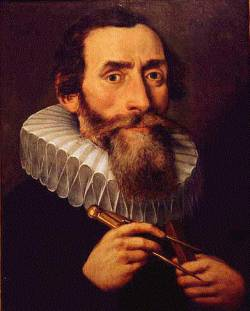
\includegraphics[width=0.2\linewidth]{screenshot001}
	\caption{Johannes Kepler (1571-1630).}
	\label{fig:JohanK}
\end{figure}

Kepler chegou às conclusões acima analisando observações astronômicas de Tycho Brahe e suas leis foram de fundamental importância para os trabalhos de Isaac Newton. A provinha em questão é dividida da seguinte forma:

\begin{enumerate}
	\item Na primeira parte, estudaremos o sistema de coordenadas polar, no qual o trabalho algébrico dos exercícios subsequentes é reduzido;
	\item No segundo tópico, analisaremos grandezas \textbf{conservadas} no tempo, um conceito de fundamental importância na física;
	\item Após isso, discutiremos seções cônicas (veja a lei \ref{enum:e1} acima);
	\item Então, verificaremos que cada lei é, de fato, respeitada pela interação gravitacional e vamos fazer uma aplicação de tudo que aprendemos para o movimento de satélites estudando a \textit{Manobra de Hohmann}!
\end{enumerate}

\bigskip

\begin{questions}

	\question \label{ques:q1}
	\textbf{A física não pode depender do sistema de coordenadas!!!} Podemos tirar vantagem disso e escolher um sistema que reduza o trabalho algébrico. Uma maneira de discriminar entre sistemas é utilizar das simetrias do problema, por exemplo, se a situação física estudada apresenta simetria esférica, nada mais justo que utilizarmos coordenadas esféricas para tratar o problema. No caso que queremos estudar, como ficará claro adiante, o sistema de coordenadas polares é útil na simplificação de contas e também na interpretação dos resultados. Nesse sistema iremos decompor os vetores em nos versores $\ehat{r}$ e $\ehat{\theta}$, sendo que os dois primeiros são relacionados com os versores cartesianos, os quais vocês estão acostumados, através das relações:
	\begin{equation}\label{eq:eretdef}
		\begin{aligned}
			\ehat{r}      & = \cos (\theta)\ehat{x} + \sin (\theta)\ehat{y} \\
			\ehat{\theta} & = - \sin(\theta)\ehat{x} + \cos(\theta)\ehat{y}
		\end{aligned}
	\end{equation}

	Considere o movimento de um planeta de massa $ m $ ao redor do sol, de massa $ M $, desconsideraremos interações gravitacionais com outros corpos, uma vez que são pequenas em comparação à do sol. Além disso consideraremos que o sol permanece praticamente imóvel na origem do sistema de coordenadas\footnote{As dimensões de ambos corpos também serão desprezadas, já que não são relevantes para a análise em questão.}, veja a figura \ref{fig:PlanetOrbit}. Em coordenadas cartesianas podemos decompor o vetor posição $\vec{r}$ da partícula da seguinte forma:
	\begin{equation}\label{eq:rcartesian}
		\vec{r}=\sqrt{x^{2}+y^{2}}\cos(\theta)\,\ehat{x}+\sqrt{x^{2}+y^{2}}\sin(\theta)\,\ehat{y}
	\end{equation}

	\begin{figure}[H]
		\centering
		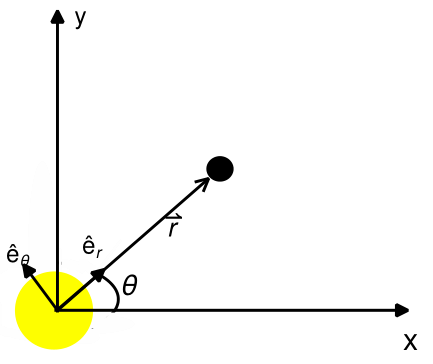
\includegraphics[width=0.4\linewidth]{screenshot002}
		\caption{Planeta de massa $ m $, orbitando o sol.}
		\label{fig:PlanetOrbit}
	\end{figure}

	\begin{parts}
		\part \label{part:q1a} Escreva \ref{eq:rcartesian} no sistema de coordenadas polares, ou seja, em termos de $ \ehat{r},\ehat{\theta} $ e do módulo de $ \envert{\vec{r}}\equiv r $.

		\begin{solution}

			\begin{multi}
				Sendo
				\begin{gather*}
					\cos\theta=\dfrac{x}{r}\implies x=r\cos\theta\\
					\sin\theta=\dfrac{y}{r}\implies y=r\sin\theta
				\end{gather*}

				\nach

				\centering
				\begin{tikzpicture}
					\draw[->] (-0.5,0) -- (2,0) node[right] {$ x $};
					\draw[->] (0,-0.5) -- (0,2) node[above] {$ y $};

					\draw[thick] (0,0) -- node[below] {$ x $} (1.5,0) -- node[right] {$ y $} (1.5,1.5) -- node[rotate=45,above] {$ r $} (0,0);

					\coordinate (O) at (0,0);
					\coordinate (r) at (1,1);
					\coordinate (x) at (1,0);

					\pic[draw=black, angle radius=15pt,angle eccentricity=1,"$ \theta $" {xshift=5pt,yshift=1pt}] {angle=x--O--r};
				\end{tikzpicture}
			\end{multi}

			Tomando $ \sqrt{x^{2}+y^{2}} $, temos:
			\begin{align*}
				\sqrt{x^{2}+y^{2}} & =\sqrt{\del{r\cos\theta}^{2}+\del{r\sin\theta}^{2}} \\
				                   & =\sqrt{r^{2}\del{\cos^{2}\theta+\sin^{2}\theta}}    \\
				\intertext{pela relação fundamental da trigonometria:}
				                   & =\sqrt{r^{2}\cdot1}=r\stackrel{!}{\geqslant}0
			\end{align*}
			Daí, temos que $ \vec{r}=r\cos\theta\,\ehat{x}+r\sin\theta\,\ehat{y}$. Agora basta nos livrarmos dos vetores unitários cartesianos.

			\begin{multi}
				Analisando o triângulo de hipotenusa unitária $ \ehat{r} $, temos:
				\begin{equation}\label{eq:ehatr}
					\ehat{r}=\ehat{x}\cos\theta+\ehat{y}\sin\theta
				\end{equation}
				Definindo $ \ehat{\theta} $ como perpendicular à $\ehat{r}$, temos
				\begin{equation}\label{eq:ehatt}
					\ehat{\theta}=-\ehat{x}\sin\theta+\ehat{y}\cos\theta
				\end{equation}
				substituindo, temos:

				\nach

				\centering
				\begin{tikzpicture}[scale=0.9]
					\coordinate (O) at (0,0);

					\draw[->] (-0.5,0) -- (2.5,0) node[right] {$ x $} coordinate (x);
					\draw[->] (0,-0.5) -- (0,2.5) node[above] {$ y $};

					\draw[-Latex, thick] (0,0) -- node[below] {$ \ehat{x} $} (2,0);

					\draw[-Latex, thick] (0,0) -- node[left] {$ \ehat{y} $} (0,2);

					\draw[-Latex, thick] (0,0) -- node[rotate=60,pos=0.7,above] {$ \ehat{r} $} (60:2) coordinate (r);

					\draw[dashed] (r-|O) -- (r) -- (r|-O);

					\pic[draw=black, angle radius=15pt,angle eccentricity=1,"$ \theta $" {xshift=5pt,yshift=1pt}] {angle=x--O--r};

					\begin{scope}[shift={(5,0)}]
						\coordinate (Op) at (0,0);

						\draw[->] (-2,0) -- (2.5,0) node[right] {$ x $} coordinate (xp);
						\draw[->] (0,-0.5) -- (0,2.5) node[above] {$ y $};

						\draw[-Latex, thick] (0,0) -- node[below] {$ \ehat{x} $} (2,0);

						\draw[-Latex, thick] (0,0) -- node[above left] {$ \ehat{y} $} (0,2);

						\draw[-Latex, thick] (0,0) -- node[rotate=60,pos=0.7, above] {$ \ehat{r} $} (60:2) coordinate (rp);

						\draw[-Latex, thick] (0,0) -- node[rotate=-30,pos=0.4,above] {$ \ehat{\theta} $} (150:2) coordinate (t);

						\draw[dashed] (t-|Op) -- (t) -- (t|-Op);

						\pic[draw=black, angle radius=15pt,angle eccentricity=1,"$ \theta $" {xshift=5pt,yshift=1pt}] {angle=xp--Op--rp};
						\dotMarkRightAngle[size=6pt](rp,Op,t);
					\end{scope}
				\end{tikzpicture}
			\end{multi}
			\begin{equation}\label{eq:r}
				\vec{r}=r\del{\ehat{x}\,\cos\theta+\ehat{y}\,\sin\theta}=r\,\ehat{r}
			\end{equation}
		\end{solution}

		\part \label{part:q1b} Calcule as seguintes derivadas e expresse-as em coordenadas polares:
		\begin{equation}\label{eq:ddtpolar}
			\dod{\ehat{r}}{t}\equiv \dot{\ehat{r}},\quad \dod{\ehat{\theta}}{t}\equiv \dot{\ehat{\theta}}
		\end{equation}

		\begin{solution}
			Derivando \ref{eq:ehatr}, temos:
			\begin{align}
				\dod{\ehat{r}}{t} & =\dot{\ehat{r}}=\del{\ehat{x}\cos\theta+\ehat{y}\sin\theta}'\nonumber                                                \\
				                  & =\ehat{x}\dot{\theta}\del{\cos\theta}'+\ehat{y}\dot{\theta}\del{\sin\theta}'\nonumber                                \\
				                  & =\dot{\theta}\del{\ehat{x}\del{-\sin\theta}+\ehat{y}\del{\cos\theta}}=\dot{\theta}\,\ehat{\theta}\label{eq:ehatrdot}
			\end{align}
			Derivando \ref{eq:ehatt}, temos:
			\begin{align}
				\dod{\ehat{\theta}}{t} & =\dot{\ehat{\theta}}=\del{-\ehat{x}\sin\theta+\ehat{y}\cos\theta}'\nonumber                                      \\
				                       & =-\ehat{x}\dot{\theta}\del{\sin\theta}'+\ehat{y}\dot{\theta}\del{\cos\theta}'\nonumber                           \\
				                       & =-\dot{\theta}\del{\ehat{x}\del{\cos\theta}+\ehat{y}\del{\sin\theta}}=-\dot{\theta}\,\ehat{r}\label{eq:ehattdot}
			\end{align}
		\end{solution}

		\part \label{part:q1c} Utilizando os resultados obtidos em \ref{eq:ddtpolar} calcule os vetores velocidade e aceleração do planeta. Exprima a resposta no sistema de coordenadas polar.

		\begin{solution}
			Munidos de \ref{eq:r}, \ref{eq:ehatrdot} e \ref{eq:ehattdot}, tomemos $ \dot{\vec{r}} $:
			\begin{equation}\label{eq:dotr}
				\dot{\vec{r}}=\dot{r}\cdot\ehat{r}+r\cdot\dot{\ehat{r}}=\dot{r}\cdot\ehat{r}+r\cdot\dot{\theta}\cdot\ehat{\theta}
			\end{equation}
			tomando, agora, $ \ddot{\vec{r}} $:
			\begin{align}
				\ddot{\vec{r}} & =\del{\dot{\vec{r}}}'=\del{\dot{r}\cdot\ehat{r}+r\cdot\dot{\theta}\cdot\ehat{\theta}}'\nonumber                                                                                                         \\
				               & =\ddot{r}\cdot\ehat{r}+\dot{r}\cdot\dot{\ehat{r}}+\dot{r}\cdot\dot{\theta}\cdot\ehat{\theta}+r\del{\ddot{\theta}\cdot\ehat{\theta}+\dot{\theta}\cdot\dot{\ehat{\theta}}}\nonumber                       \\
				\intertext{substituindo \ref{eq:ehatrdot} e \ref{eq:ehattdot}, e adotando $ \dot{a}^{2}:=\dot{a}\cdot\dot{a} $, temos}
				               & =\ddot{r}\cdot\ehat{r}+\dot{r}\cdot\dot{\theta}\cdot\ehat{\theta}+\dot{r}\cdot\dot{\theta}\cdot\ehat{\theta}+r\del{\ddot{\theta}\cdot\ehat{\theta}-\dot{\theta}\cdot\dot{\theta}\cdot\ehat{r}}\nonumber \\
				\ddot{\vec{r}} & =\del{\ddot{r}-r\cdot\dot{\theta}^{2}}\ehat{r}+\del{2\dot{r}\cdot\dot{\theta}+r\cdot\ddot{\theta}}\ehat{\theta}\label{eq:ddotr}
			\end{align}
		\end{solution}
	\end{parts}

	\medskip

	\question \label{ques:q2} O momento angular $\vec{L}$ é definido da seguinte forma:
	\begin{equation}\label{eq:angMommentum}
		\vec{L}=\vec{r}\times\vec{p}
	\end{equation}
	Onde $\vec{p}$ e $\vec{r}$ são, respectivamente, o momento e a posição do planeta.

	\begin{parts}
		\part \label{part:q2a} Calcule a derivada do momento angular $ \dod{\vec{L}}{t} $.

		\paragraph{Dica:} O produto vetorial satisfaz a regra do produto para derivadas.

		\begin{solution}
			Pela dica, sabemos que
			\[ \dod{\vec{L}}{t}=\dod{\vec{r}}{t}\times \vec{p}+\vec{r}\times\dod{\vec{p}}{t} \]
			sendo o momento $ \vec{p}=m\,\dot{\vec{r}} $, temos:
			\begin{align*}
				\dod{\vec{L}}{t} & =\dot{\vec{r}}\times \vec{p}+\vec{r}\times\dot{\vec{p}}                                                                                                                                  \\
				\intertext{como um vetor é paralelo a si mesmo, temos}
				                 & =\cancelto{0}{\dot{\vec{r}}\times \del{m\,\dot{\vec{r}}}}+\vec{r}\times\del{m\,\dot{\vec{r}}}'                                                                                           \\
				                 & =m\,\vec{r}\times\ddot{\vec{r}}                                                                                                                                                          \\
				\intertext{por \ref{eq:ddotr}, temos}
				                 & =m\,\dot{\vec{r}}\times\del{\del{\ddot{r}-r\cdot\dot{\theta}^{2}}\ehat{r}+\del{2\dot{r}\cdot\dot{\theta}+r\cdot\ddot{\theta}}\ehat{\theta}}                                              \\
				                 & =m\,\del{\cancelto{0}{\dot{\vec{r}}\times\del{\del{\ddot{r}-r\cdot\dot{\theta}^{2}}\ehat{r}}}+\dot{\vec{r}}\times\del{\del{2\dot{r}\cdot\dot{\theta}+r\cdot\ddot{\theta}}\ehat{\theta}}} \\
				                 & =m\del{2\dot{r}\cdot\dot{\theta}+r\cdot\ddot{\theta}}\,\dot{\vec{r}}\times\ehat{\theta}                                                                                                  \\
				\intertext{por \ref{eq:ehatr}, \ref{eq:ehatt} e \ref{eq:r}, temos}
				                 & =m\,r\del{2\dot{r}\cdot\dot{\theta}+r\cdot\ddot{\theta}}\,\begin{vmatrix}
					\ehat{x}    & \ehat{y}   & \ehat{z} \\
					\cos\theta  & \sin\theta & 0        \\
					-\sin\theta & \cos\theta & 0
				\end{vmatrix}                                                                                                     \\
				                 & =m\,r\del{2\dot{r}\cdot\dot{\theta}+r\cdot\ddot{\theta}}\del{\ehat{x}\del{0\sin\theta-0\cos\theta}-\ehat{y}\del{0\cos\theta+0\sin\theta}+\ehat{z}\del{\cos^{2}\theta+\sin^{2}\theta}}    \\
				\intertext{pela relação fundamental da trigonometria}
				                 & =m\,r\del{2\dot{r}\cdot\dot{\theta}+r\cdot\ddot{\theta}}\ehat{z}
			\end{align*}
		\end{solution}

		\part \label{part:q2b} Mostre que o momento angular é conservado se atuar na partícula somente uma força central $ \vec{F}=f(r)\vec{r} $.

		\part \label{part:q2c} Considere a interação gravitacional:
		\begin{equation}\label{eq:gravForce}
			\vec{F}=-\dfrac{G\,M\,m}{r^{3}}\vec{r}
		\end{equation}

		A energia potencial gravitacional associada à força acima é\footnote{Fixamos seu valor igual a zero no infinito.}:
		\begin{equation}\label{eq:gravPot}
			U(r)=-\dfrac{G\,M\,m}{r}
		\end{equation}
		Escreva a energia mecânica total do planeta. Utilize a velocidade em coordenadas polares, como feito no item \ref{ques:q1}(\ref{part:q1c}), para escrever o resultado final em coordenadas polares.

		\part \label{part:q2d} Utilizando novamente o item \ref{ques:q1}(\ref{part:q1c}), escreva a segunda lei de Newton para o problema em questão e encontre as equações de movimento para as componentes $\ehat{r}$ e $ \ehat{\theta} $.

		\part \label{part:q2e} Calcule $ \od{E}{t} $ e use o resultado obtido em \ref{ques:q2}(\ref{part:q2d}) para mostrar que a energia é conservada.

		\part \label{part:q2f} Calcule o produto escalar $ \vec{L}\cdot\vec{r} $, o que você pode concluir desse resultado combinado com o que obteve em \ref{ques:q2}(\ref{part:q2b})? Nesse momento deve ficar claro porque podemos representar o movimento com acurácia utilizando apenas a Figura \ref{fig:PlanetOrbit}.

		\paragraph{Dica:} Lembre-se de que a equação de um plano pode ser escrita na forma $ \vec{N}\cdot\vec{r}=0 $ onde $\vec{N}$ é o vetor normal ao plano.
	\end{parts}

	\question \label{ques:q3} Agora, de posse das equações de movimento e sabendo que a situação física satisfaz a condição estabelecida por \ref{ques:q2}(\ref{part:q2f}), é necessário entendermos seções cônicas. Para isso considere o seguinte problema de geometria analítica:
	\begin{quotation}
		\itshape ``Qual o lugar geométrico descrito por um ponto móvel cuja distância à um ponto fixo tem proporção constante em relação a sua distância perpendicular à uma linha fixa ?''
		%		\par\raggedleft--- \textup{Newton}, Optics \textup{(citado por French)}
	\end{quotation}
	Para entender melhor a situação considere a Figura \ref{fig:fig3}, onde adotamos como ponto fixo, chamado foco, a origem e consideramos que a linha fixa seja a reta que passa por $ x = -d $. Sendo a distância de um ponto arbitrário (o ponto móvel do enunciado acima) ao foco $ r_1 $ e a distância dele à reta fixa $ r_2 $ (Veja a Figura \ref{fig:fig3}), responda:

	\begin{figure}[H]
		\centering
		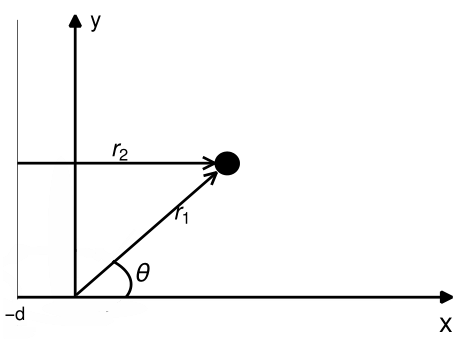
\includegraphics[width=0.5\linewidth]{screenshot003}
		\caption{Representação gráfica do problema geométrico. Note que $ r_1 $, faz o papel do módulo do raio $ r $ do exercício anterior.}
		\label{fig:fig3}
	\end{figure}

	\begin{parts}
		\part \label{part:q3a} Calcule a proporção $ r_1/r_2 $ em termos de $ r_1,\theta $ e $ d $. Note que, caso troquemos nosso ponto móvel por uma partícula ou um corpo extenso cujas dimensões podem ser desprezadas, $ r_1 $ se reduz, em coordenadas polares, ao módulo do vetor posição $ r_1 = \envert{r} $.

		\part \label{part:q3b} Queremos que o quociente $ r_1/r_2 $ seja constante igual a $ e $, chamado de excentricidade da cônica. Reescreva $ r_1 $ em termos de $ r_c = e\,d,e $ e $\theta$.

		Podemos reescrever o resultado de \ref{ques:q3}(\ref{part:q3b}) em coordenadas cartesianas, correspondendo a três situações distintas:
		\begin{enumerate}
			\item Se $ e<1 $:
			      \begin{equation}\label{eq:sit1}
				      \dfrac{\del{x-x_c}^{2}}{a^{2}}+\dfrac{y^{2}}{b^{2}}=1\,
			      \end{equation}
			      onde
			      \begin{equation}\label{eq:sit1where}
				      \begin{aligned}
					      a   & =\dfrac{r_c}{1-e^{2}} \\
					      b   & =\sqrt{1-e^{2}}\,a    \\
					      x_c & =e\,a
				      \end{aligned}
			      \end{equation}

			      A equação \ref{eq:sit1} descreve uma elipse centrada em $ \intoo{x_c,0} $, de raio maior $ a $ e raio menor $ b $ (veja a	Figura \ref{fig:ellipseGraph}).

			      \begin{figure}[H]
				      \centering
				      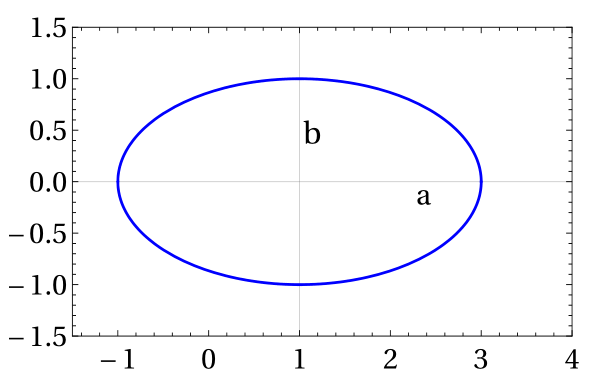
\includegraphics[width=0.5\linewidth]{screenshot004}
				      \caption{Exemplo de uma eplise com $ a = 2, b = 1 $ e $ x_c = 1 $.}
				      \label{fig:ellipseGraph}
			      \end{figure}

			\item Se $ e>1 $:
			      \begin{equation}\label{eq:sit2}
				      \dfrac{\del{x-x_c}^{2}}{a^{2}}-\dfrac{y^{2}}{b^{2}}=1\,
			      \end{equation}
			      onde
			      \begin{equation}\label{eq:sit2where}
				      \begin{aligned}
					      a   & =\dfrac{r_c}{e^{2}-1} \\
					      b   & =\sqrt{e^{2}-1}\,a    \\
					      x_c & =-e\,a
				      \end{aligned}
			      \end{equation}

			      A equação \ref{eq:sit2} descreve uma hipérbole com assíntotas intersectando em $ \intoo{x_c,0} $ (Veja a Figura \ref{fig:hyperbolaGraph}).

			      \begin{figure}[H]
				      \centering
				      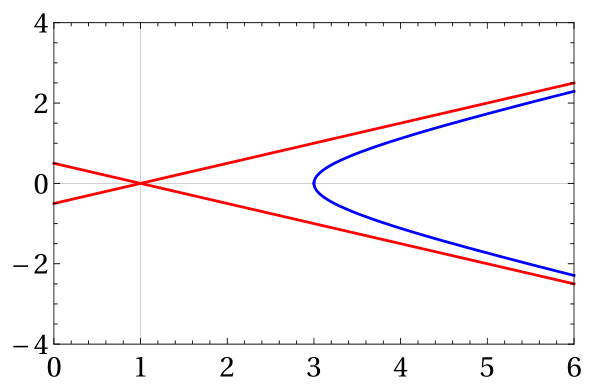
\includegraphics[width=0.5\linewidth]{screenshot005}
				      \caption{Exemplo de uma hipérbole com $ a = 2, b = 1 $ e $ x_c = 1 $. As retas vermelhas representam suas assíntotas.}
				      \label{fig:hyperbolaGraph}
			      \end{figure}

			\item Se $ e=1 $:
			      \begin{equation}\label{eq:sit3}
				      y^{2}-2r_c\del{x-x_c}=0,
			      \end{equation}
			      onde
			      \begin{equation}\label{eq:sit3where}
				      x_c=-\dfrac{r_c}{2}
			      \end{equation}

			      A equação \ref{eq:sit3}, provavelmente a mais familiar a vocês, descreve uma parábola alinhada ao eixo x que passa por $ \intoo{x_c, 0} $ (Veja Figura \ref{fig:parabolaGraph}). Temos agora todos os ingredientes necessários para derivar, de primeiros princípios, as Leis de Kepler!

			      \begin{figure}[H]
				      \centering
				      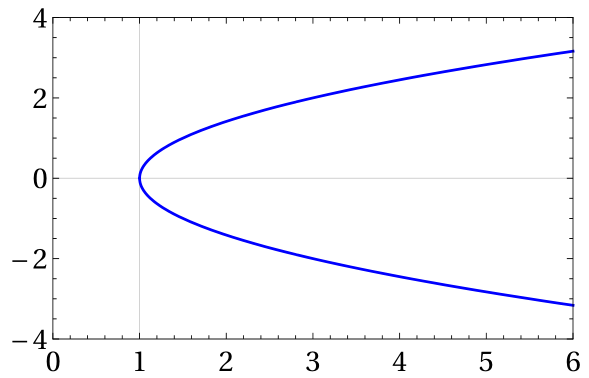
\includegraphics[width=0.5\linewidth]{screenshot006}
				      \caption{Exemplo de uma parábola alinhada ao eixo x com xc = 1.}
				      \label{fig:parabolaGraph}
			      \end{figure}
		\end{enumerate}
	\end{parts}

	\question \label{ques:q4} De volta à Figura \ref{fig:PlanetOrbit}, vamos analisar primeiramente a validade da lei \ref{enum:e2}:

	\begin{parts}
		\part \label{part:q4a} Escreva o momento angular $ \vec{L} $ em coordenadas polares.

		\paragraph{Dica:} Note que $ \ehat{r}\times\ehat{\theta}=\ehat{z} $.
		Caso você não tenha conseguido mostrar a conservação de momento angular no caso geral do exercício \ref{ques:q2}, tente mostrar que para o caso particular\footnote{Por particular queremos dizer após decompor o vetor em um sistema de coordenadas específico, uma vez que a conservação é geral e independe de sistema de coordendas.} dessa questão que, de fato, a equação
		\[ \dod{\vec{L}}{t}=\vec{0} \]
		é satisfeita.

		\paragraph{Dica:} Calcule a derivada acima e compare com a equação de movimento para a componente $ \ehat{\theta} $.

		\part \label{part:q4b} Vocês verão no futuro que a área de uma elipse pode ser calculada pela integral dupla
		\[ A=\int_{0}^{2\pi}\dif\theta\int_{0}^{r(\theta)}r'\dif r' \]
		E poderão tirar as mesmas conclusões que iremos chegar analisando o limite a seguir:

		Considere a Figura \ref{fig:ellipseArc}, que representa um arco de uma elipse. Se $ \Delta\theta\ll 1 $, podemos aproximar a área do arco pela área de um triângulo:
		\[ \Delta A=\dfrac{r^{2}\Delta\theta}{2} \]

		\begin{figure}[H]
			\centering
			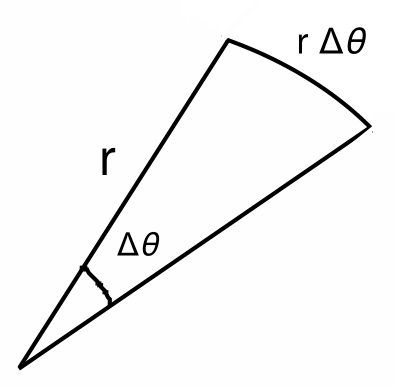
\includegraphics[width=0.4\linewidth]{screenshot007}
			\caption{Arco de uma elipse.}
			\label{fig:ellipseArc}
		\end{figure}

		Calcule $ \lim\limits_{\Delta t\to0}\Delta A/\Delta t $ e compare com o momento angular (item \ref{ques:q2}(\ref{part:q2a})). O que você pode concluir sobre a taxa de variação da área? É compatível com a segunda lei de Kepler?

		\part \label{part:q4c} Agora considere a equação de movimento na direção radial (item \ref{ques:q2}(\ref{part:q2d})). Utilize a troca de variáveis $ r(t)=u^{-1}(t) $ e mostre que:
		\begin{gather*}
			\dot{r}=-\dfrac{\dot{u}}{u^{2}}=-r^{2}\dod{u}{\theta}\dod{\theta}{t}=-h\dod{u}{\theta}\\
			\ddot{r}=-\dod[2]{u}{\theta}\dot{\theta}=-u^{2}\,h^{2}\dod[2]{u}{\theta}
		\end{gather*}
		Onde $ h=L/m $ é o momento angular por unidade de massa do planeta e utilizamos a regra da cadeia para obter as últimas igualdades. Também adotamos a notação menos carregada $ \envert{\vec{L}} \equiv L $.

		\part \label{part:q4d} Com isso, mostre que a equação radial pode ser transformada em \[ \dod[2]{u}{\theta}+u=\dfrac{G\,M}{h^{2}}. \]

		\part \label{part:q4e} Confira que a seguinte expressão é solução da equação diferencial acima:
		\begin{equation}\label{eq:difSol}
			u(\theta)=\dfrac{G\,M}{h^{2}}\del{1-e\cos\del{\theta-\theta_0}},
		\end{equation}
		onde $ \theta_0 $ e $ e $ são constantes. Podemos tomar, sem perda de generalidade, $ \theta_0=0 $, de forma que a solução $ r(\theta) $ é dada por
		\begin{equation}\label{eq:difSol2}
			r(\theta)=\dfrac{r_c}{1-e\cos(\theta)}
		\end{equation}
		onde $ r_c=h^{2}/(G\,M) $. Compare essa equação com o resultado obtido em \ref{ques:q3}(\ref{part:q3b}). Essa é a equação de uma cônica confocal com a origem (no caso da dinâmica celeste estamos supondo que a origem do sistema de coordenadas está fixa no sol). Para o caso $ e < 1 $ essa equação descreve uma elipse. Dado que as outras cônicas não descrevem movimentos limitados (reflita o porquê disso), tire suas conclusões sobre a mecânica celeste e confronte com \ref{enum:e1}.

		\part \label{part:q4f} Suponha que $ a $ e $ b $ sejam, respectivamente, o valor do raio maior e menor da elipse. A área da elipse é então dada por
		\[ A = \pi\,a\,b \]

		No item \ref{ques:q4}(\ref{part:q4b}) foi calculada a taxa de variação da área no tempo. O período do movimento pode ser calculado considerando o tempo necessário para varrer a área total da elipse a uma taxa constante $ \od{A}{t} $:
		\[ T=\dfrac{A}{\dod{A}{t}}. \]

		Calcule o valor acima e utilize os resultados resumidos em \ref{eq:sit1where} e que $ r_c=h^{2}/(GM) $ para escrever o quadrado do período em função apenas do raio maior $ a $. Enfim, mostramos que a lei \ref{enum:e3} vale!
	\end{parts}

	\question \label{ques:q5} Todo formalismo desenvolvido até esse ponto pode ser utilizado para entendermos a \textit{manobra de Hohmann}. Considere que um satélite artificial descreve uma órbita circular de raio $ r_1 $ ao redor do sol e queremos fazer com que ele passe a descrever uma órbita circular $ r_2 > r_1 $. Para tal, vamos utilizar uma órbita elíptica para fazer o translado entre as órbitas circulares (veja Figura \ref{fig:HohmannMan}).

	\begin{parts}
		\part \label{part:q5a} Utilize seu resultado de \ref{ques:q4}(\ref{part:q4c}) e a substituição $ r = u^{-1} $ para escrever a energia por unidade de massa:

		\begin{figure}[H]
			\centering
			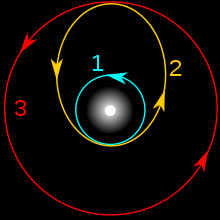
\includegraphics[width=0.4\linewidth]{screenshot008}
			\caption{A manobra de transferência entre órbitas circulares de Hohmann.}
			\label{fig:HohmannMan}
		\end{figure}
		\begin{equation}\label{eq:epsilonThing}
			\varepsilon=\dfrac{E}{m}=\dfrac{h^{2}}{2}\del{\del{\dod{u}{\theta}^{2}+u(\theta}^{2}-2u(\theta)u_c}
		\end{equation}

		\part \label{part:q5b} Substitua a solução $ u(\theta) $ de \ref{eq:difSol} e mostre que
		\[ \varepsilon=\dfrac{u_c\,h^{2}}{2}\del{e^{2}-1}=\dfrac{G\,M}{2r_p}\del{e-1}, \]
		onde $ u_c = r_e^{-1} $ e $ r_p $ é chamado periélio, a distância mais próxima que o planeta chega do sol em toda sua órbita ($ \theta = \pi $ em \ref{eq:difSol2}):
		\begin{equation}\label{eq:rperihelium}
			r_p=\dfrac{r_c}{1+e}=a\del{1-e}
		\end{equation}
		Discuta o sinal de $ \varepsilon $ para cada uma das cônicas $ e < 1, e = 1 $ e $ e > 1 $. Você se lembra da primeira provinha do átomo de Bohr\footnote{Essa provinha foi aplicada apenas para o pessoal da Geofísica, deixaremos ela disponível na página do curso no moodle para quem quiser olhar.}? Discutimos que a energia gravitacional deveria ser negativa para estados que formam órbitas uma vez que o zero da energia potencial foi fixado no infinito. Aqui você pode vislumbrar que esse resultado é, de fato, consistente. Como você mostrou anteriormente, a energia é conservada, logo basta calcularmos seu valor para um ponto e ele deve ser o mesmo para todos os instantes subsequentes.

		\part \label{part:q5c} Use \ref{eq:rperihelium} para mostrar que podemos escrever a energia como função apenas do raio maior a:
		\begin{equation}\label{eq:epsilonCircle}
			\varepsilon=-\dfrac{G\,M}{2a}
		\end{equation}
		Para o movimento circular, temos que $ \dot{r}=0 $ e que $ a = b = r_c $, sendo agora justificado o porquê de adotamos o índice c durante todo o exercício.

		\part \label{part:q5d} Mostre que, para órbitas circulares, levando em conta a conservação de energia e utilizando \ref{eq:epsilonCircle}, a velocidade tangencial é dada por:
		\[ v_c=\sqrt{\dfrac{G\,M}{r_c}} \]

		\part \label{part:q5e} Faça o mesmo raciocínio para o momento em que o planeta se encontra no periélio $ r_p $ e mostre que:
		\begin{equation}\label{eq:vpvcRatio}
			\dfrac{v_p}{v_c}=\sqrt{1+e}
		\end{equation}

		\paragraph{Dica:} Note que no periélio também temos que $ \dot{r}=0 $.

		Analogamente, no afélio --- maior distância possível entre o planeta e o sol --- temos:
		\begin{equation}\label{eq:aphelium}
			r_a = a(1 + e)
		\end{equation}
		Podemos mostrar que:
		\begin{equation}\label{eq:vavcRatio}
			\dfrac{v_a}{v_c}=\sqrt{1-e}
		\end{equation}
		Ufa! Agora nos resta apenas interpretar os resultados acima. Suponha que nosso satélite esteja numa órbita circular de raio $ r_1 $ e queremos transferí-lo para um órbita circular de raio $ r_2 > r_1 $. Nós podemos realizar esse feito colocando o satélite temporariamente em uma órbita elíptica na qual o periélio é a distância $ r_1 $ e o afélio é a distância $ r_2 $. Neste caso, a excentricidade será dada por:
		\[ e=\dfrac{r_2-r_1}{r_2+r_1} \]

		De acordo com o resultado de \ref{eq:vpvcRatio}, podemos transferir o satélite de sua órbita circular inicial para a órbita elíptica discutida acima se aumentarmos sua velocidade tangencial (ligando os motores do satélite durante um intervalo de tempo, de forma que causem a aceleração necessária) por um fator
		\[ \kappa_1=\sqrt{1+e} \]

		Uma vez que o satélite está percorrendo a trajetória da elipse, aguardamos o instante no qual ele atinge seu afélio (percorrendo metade da órbita) para reativar os motores e mudar a velocidade, segundo \ref{eq:vavcRatio}, por um fator
		\begin{equation}\label{eq:kappa2}
			\kappa_2=\dfrac{1}{\sqrt{1-e}}
		\end{equation}

		Então o satélite estará com a velocidade tangencial compatível para realizar o movimento circular e assim permanecerá enquanto estiver sob ação apenas da força gravitacional! Legal, não?

		\part \label{part:q5f} \textbf{Para provocar...} Imagine que dormimos no ponto após ligar os motores e deixamos o dispositivo ligado de maneira que em \ref{eq:vpvcRatio} a nova velocidade tangencial satisfaça:
		\[ \dfrac{v_t}{v_c}>\sqrt{2} \]
		O que ocorrerá em momentos subsequentes?

		\begin{figure}[H]
			\centering
			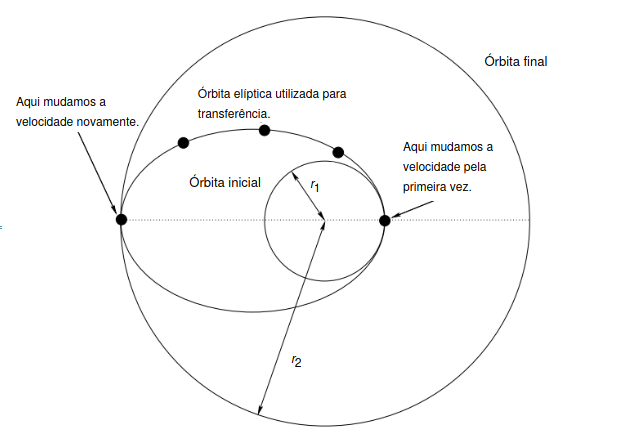
\includegraphics[width=0.7\linewidth]{screenshot009}
			\caption{Representação da situação estudada.}
			\label{fig:situation}
		\end{figure}

	\end{parts}
\end{questions}
\end{document}
